%! TEX TS-program = lualatex
%! TeX root = doc/slides.tex

\documentclass[aspectratio=169]{beamer}

\newcommand{\names}{Gabriel \textsc{Doriath Döhler}, Constantin \textsc{Gierczak--Galle}}

\title{"Craft your IC"\\Learning hardware design in
Minecraft\footnote{\tiny{}\reproduce}\\\small{} École Normale Supérieure, Paris (ENS Ulm)}
\author{\names}
\institute{FSiC $2023$}
\date{July $12$, $2023$}

\usepackage{fontspec}
\setmonofont{FreeMono}
\usepackage{amsmath}
\usepackage{listings}
\usepackage{xcolor}
\usepackage{qrcode}
\usepackage{caption}

\newcommand{\rv}{\texttt{RISC-V}}
\newcommand{\vrv}{\texttt{V-\rv}}
\newcommand{\hw}{HW}
\newcommand{\rvlink}{https://wiki.f-si.org/index.php?title=Learning_hardware_design_in_the_video_game_Minecraft}

\setcounter{tocdepth}{1}

\begin{document}
\beamertemplatenavigationsymbolsempty
\addtobeamertemplate{navigation symbols}{}{%
	\usebeamerfont{footline}%
	\usebeamercolor[fg]{footline}%
	\hspace{1em}%
	\insertframenumber/\inserttotalframenumber
}

\maketitle

\begin{frame}[fragile]
	\frametitle{Story time}
	\begin{figure}
		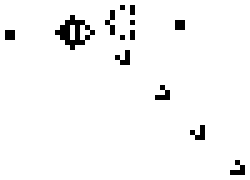
\includegraphics[width=.5\textwidth]{imgs/game_of_life.png}
		\caption*{Conway's game of life, by Lucas Vieira - Own work, CC BY-SA 3.0, https://commons.wikimedia.org/w/index.php?curid=101736}
	\end{figure}

	% game of life turing machine
	% borrow computational construct from the game
	% sysnum CPU, cst1 + gdd idée MC
	% but there is one problem: know that we had the idea, we had to do it, somehow the TAs accepted
	% but why???
	% - Minecraft is a good interactive tool to learn hardware concepts
	% - BUT IT'S ALSO VERY FUN
\end{frame}

\begin{frame}[fragile]
	\frametitle{Table of Contents}
	\tableofcontents
\end{frame}

\section{Logic circuits in Minecraft}

 {
  \usebackgroundtemplate{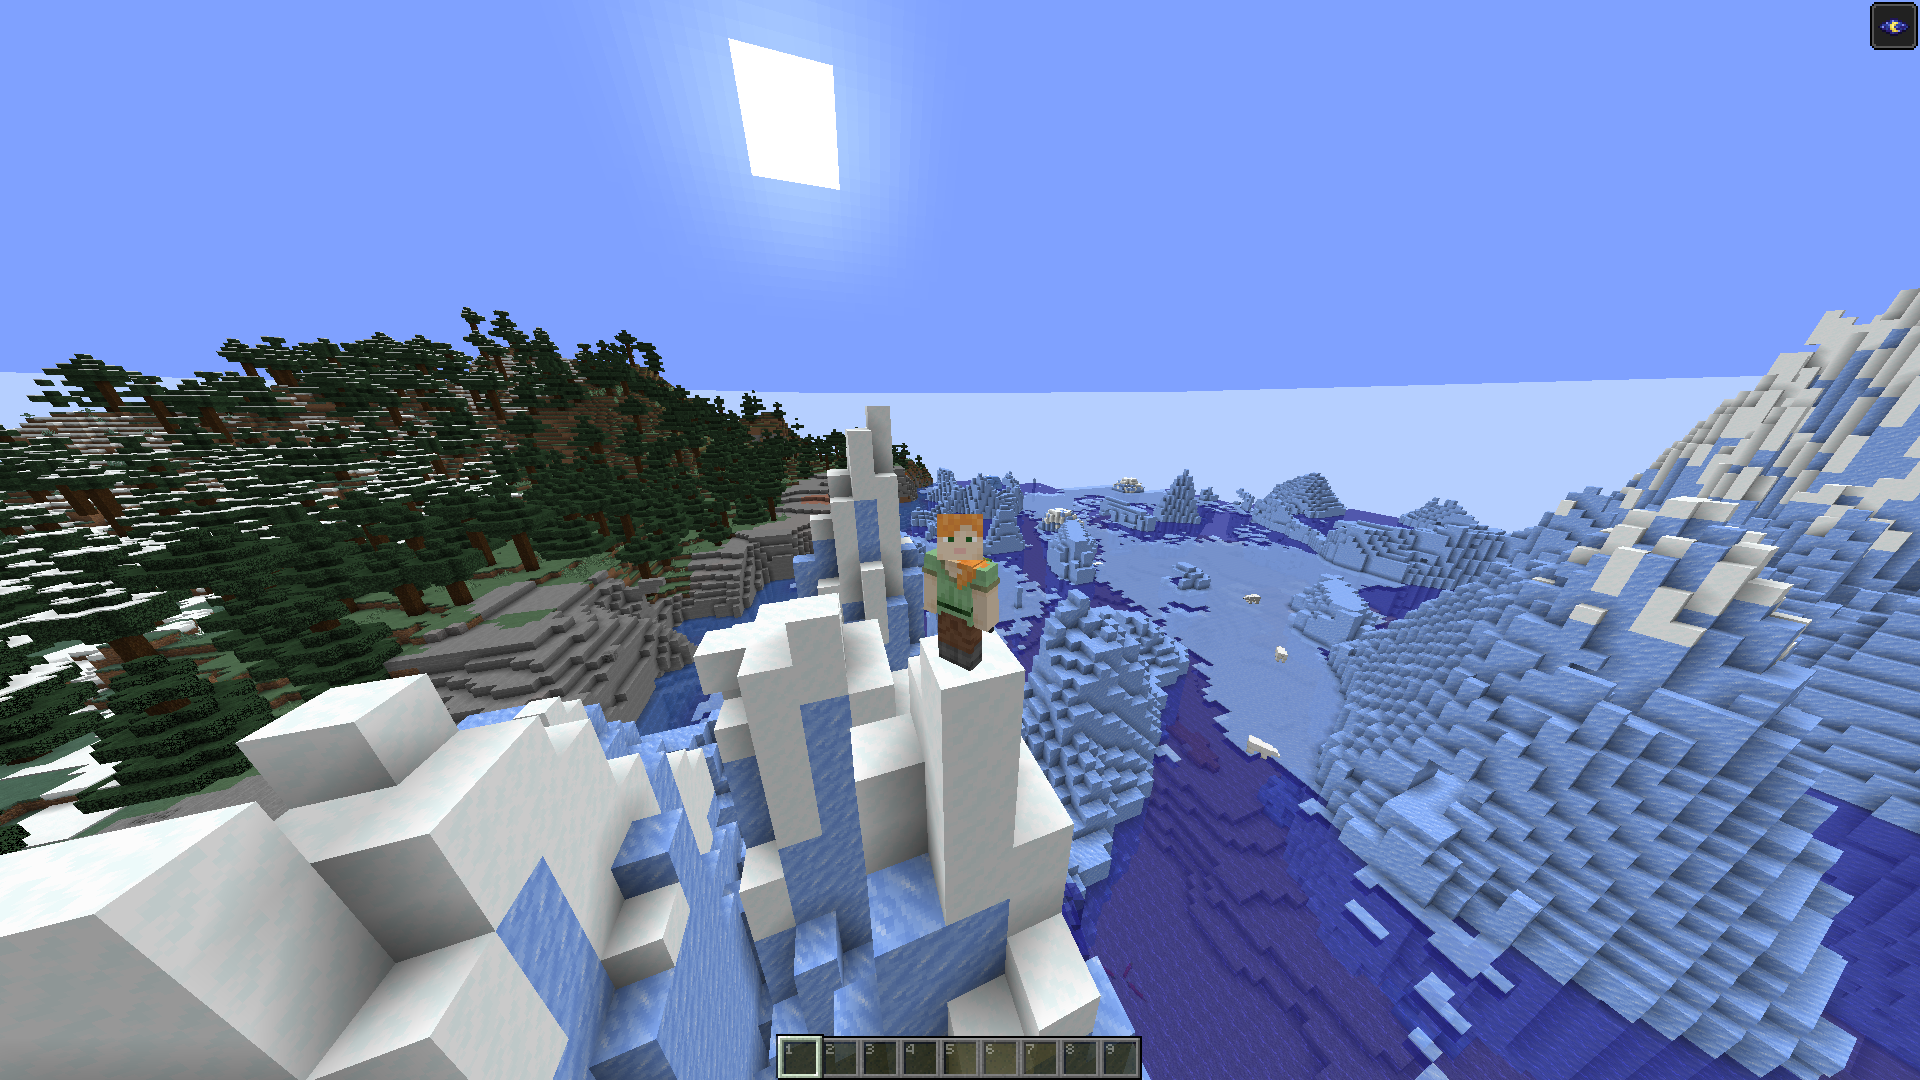
\includegraphics[width=\paperwidth]{imgs/minecraft.png}}
  \begin{frame}[plain]
	  % block game owned by microsoft (not open source but reverse friendly)
	  % a player moves and can place/delete cubes (called blocks) in a grid
  \end{frame}
 }

\begin{frame}
	\frametitle{Minecraft Redstone}

	\begin{columns}
		\begin{column}{0.5\textwidth}
			Redstone = equivalent of electronics
			\begin{itemize}
				\item<1->{Lever = player input}
				\item<1->{Lamp = output}

				\item<2->{Redstone = wires}

				\item<3->{Torch = NOT gate}
				\item<3->{1 tick = 0.1 sec}

				\item<4->{Repeater}
				\begin{itemize}
					\item<4->{delay element}
					\item<4->{diode}
					\item<4->{amplifier}
					\item<4->{memory cell}
				\end{itemize}

				\item<4->{Many more redstone components...}
				\item<8>{MC = netlist simulator for 4-bit valued signals}
			\end{itemize}
		\end{column}
		\begin{column}{0.5\textwidth}
			\begin{center}
				\includegraphics<1>[width=0.9\textwidth]{imgs/lamp.png}

				\includegraphics<2>[width=0.4\textwidth]{imgs/wire.png}
				\includegraphics<2>[width=0.4\textwidth]{imgs/or_gate.png}
				\includegraphics<2>[width=0.4\textwidth]{imgs/fanout.png}

				\includegraphics<3>[width=0.7\textwidth]{imgs/torch_on.png}
				\includegraphics<3>[width=0.7\textwidth]{imgs/torch_off.png}

				\includegraphics<4>[width=0.4\textwidth]{imgs/repeater_delay_off.png}
				\includegraphics<4>[width=0.4\textwidth]{imgs/repeater_delay_on.png}
				\includegraphics<4>[width=0.5\textwidth]{imgs/repeater_diode.png}

				\includegraphics<5>[width=0.9\textwidth]{imgs/repeater_clock.png}

				\includegraphics<6>[height=0.8\textheight]{imgs/power_strength.png}
				\includegraphics<6>[height=0.8\textheight]{imgs/repeater_amplifier.png}

				\includegraphics<7>[width=0.9\textwidth]{imgs/repeater_memory_cell.png}
			\end{center}
		\end{column}
	\end{columns}

	% can't have 4 meters of cables like in tiny tapeout

\end{frame}

% \begin{frame}
% 	\frametitle{Minecraft Redstone: unusual behavior}
%
% 	\begin{columns}
% 		\begin{column}{0.5\textwidth}
% 			\begin{itemize}
% 				\item<1->Comparators =\\ weird transistors with 2 modes:
% 				\begin{itemize}
% 					\item<1->{Compare mode transmits iff\\ main input > side input}
% 					\item<1->{Substract =\\ max(0, main input - side input)}
% 				\end{itemize}
% 				\item<2->{Slab = instant diode}
% 			\end{itemize}
% 		\end{column}
% 		\begin{column}{0.5\textwidth}
% 			\begin{center}
% 				\includegraphics<1>[width=0.7\textwidth]{imgs/cmp.png}
% 				\includegraphics<1>[width=0.7\textwidth]{imgs/cmp_sub.png}
%
% 				\includegraphics<2>[width=0.9\textwidth]{imgs/slab.png}
% 			\end{center}
% 		\end{column}
% 	\end{columns}
% 	% skip barrels
%
% 	MC = netlist simulator for 4-bit valued signals
% \end{frame}

% \begin{frame}
% 	\frametitle{Building Circuits!}
% 	we already built a clock and a memory cell
% 	example of simple circuits
% 	half adder (in game)
% 	MUX/DEMUX?
% 	cool minecraft tech: CCA adder (Yap7 + Magic:\^ (2014)))
% 	$$cc_i = carry_cancel_i = cancel_i = a_i nand b_i = not propagate$$
% 	$$g_i = generate_i = a_1 and b_i$$
% 	$$c_{i+1} = (not cancel_i) and (generate_i or ((not cancel_{i-1}) and (generate_{i-1} or ...)))$$
% 	$$= ((not cancel_i) and generate_i) or ((not cancel_i) and (not cancel_{i-1}) and generate_{i-1}) or ...$$
% 	$$= sum_{j=0}^{i} generate_{j} and prod_{k=j}^{i} ¬cancel_k$$
% 	$$slabTower_{g_i} = max power strength_{j=0}^{i-1} generate_j$$
% 	$$slabTower_{cc_i} = max power strength_{j=0}^{i-1} cc_j$$
% 	works because a carry that is later canceled will have less power strength on th towers
% 	$$c_{i+1} = slabTower_{g_i} > slabTower_{cc_i}$$
% 	$$c_0 = carry_in$$
% 	$$a_n = b_n = 0$$
% 	$$o_i = a_i xor b_i xor c_i$$
% 	cancel doesn't have to be accurate (use NOR)
%
% 	7 ticks design (5 tick possible?)
% 	fully synchronized
% 	pipeline every 1 or 2 ticks
% \end{frame}

\begin{frame}
	\frametitle{Minecraft vs "Real" Hardware: what's different?}
	A few oddities
	\begin{itemize}
		\item Power strength logic
		\item Instant diodes
	\end{itemize}
	Fewer tooling
	\begin{itemize}
		\item HDL
		\item Version control
		\item GTKWave
		\item Test framework
	\end{itemize}
	Constraining physical layer
	\begin{itemize}
		\item Performance => short wires => compact
		\item Large wires => compact is hard
	\end{itemize}
\end{frame}

\section{"Craft your IC" Design and ISA}

% note for cst1: i would talk about:
% - ISA choice (why not RISV-V?)
% - debuging (replay mod)
% - wirering the different parts is a challenge
% - decoding instruction is trivial because of instruction length
% - simple pipeline (wave pipeline) (not done yet)
% - the things you already mention

\begin{frame}
	\frametitle{Roadmap}

	\begin{itemize}
		\item Design an ISA
		\item Implement it in Minecraft
		\item Build a toolchain around it
		\item Do some formal verification
		\item Discover the existing tools and community along the way
	\end{itemize}


\end{frame}

\begin{frame}
	\frametitle{Instruction Set Architecture}
	%\vrv
	%\texttt{(Very-RISC)-V}

	$32$-bit instruction words

	$8$-bit registers:

	\begin{itemize}
		\item \texttt{\%0}: $00000000$ -- like \rv{}
		\item \texttt{\%1}: $11111111$ -- for $1$--op \texttt{inc}
		      \texttt{dec}, \texttt{not}
		\item \texttt{\%2}-\texttt{\%14}: GP registers
		\item \texttt{\%15}: Random register
	\end{itemize}

	\pause

	Instructions:
	\begin{itemize}
		\item \textbf{Binops}: \texttt{add}, \texttt{sub}, \texttt{or},
		      \texttt{xor}: $3$ register operands
		\item \textbf{Jumps}: unconditional or
		      \texttt{oveflow}/\texttt{negative}/\texttt{zero}
		\item \texttt{loadi}
		\item \textbf{RAM}: load \& store
		\item \texttt{print}: print byte to 7-segment display
	\end{itemize}
\end{frame}

\subsection{A $8$-bit CPU}

{
	\usebackgroundtemplate{\includegraphics[width=\paperwidth]{imgs/cpu2.png}}
	\begin{frame}[plain]
		% block game owned by microsoft (not open source but reverse friendly)
		% a player moves and can place/delete cubes (called blocks) in a grid
	\end{frame}
}
% Harvard architecthture (separate ROM and RAM)
% 8 bits because max power strength is 15 so the ALU towers do not need repeaters
\begin{frame}
	\frametitle{ROM}% and PC}
	\begin{columns}
		\begin{column}{0.4\textwidth}
			\begin{itemize}
				\item $128$ instructions ROM
				\item Bits encoded as presence/absence of power blocks in a grid
			\end{itemize}
		\end{column}
		\begin{column}{0.6\textwidth}
			\begin{center}
				\includegraphics<1>[width=0.8\textwidth]{imgs/rom.png}
				%\includegraphics<2->[width=0.325\textwidth]{imgs/pc.png}

				\framesubtitle<1>{ROM bank}
				%\framesubtitle<2->{Program Counter}
			\end{center}
		\end{column}
	\end{columns}
\end{frame}

\begin{frame}
	\frametitle{Registers}
	\begin{columns}
		\begin{column}{0.5\textwidth}
			\begin{itemize}
				\item Tileable design for easier development
				\item All registers doubled for dual--read
				\item \texttt{\%0} and \texttt{\%1} hard-wired
				\item \texttt{\%15} random register uses Minecraft randomizers
			\end{itemize}
		\end{column}
		\begin{column}{0.5\textwidth}
			\begin{center}
				\includegraphics<1>[width=0.9\textwidth]{imgs/register_slice.png}
				\includegraphics<2->[width=0.9\textwidth]{imgs/register_file.png}

				\framesubtitle<1>{Register}
				\framesubtitle<2->{Register file}
			\end{center}
		\end{column}
	\end{columns}
\end{frame}

\begin{frame}
	\frametitle{ALU}
	\begin{columns}
		\begin{column}{0.4\textwidth}
			\begin{itemize}
				% TODO
				\item Tileable design
				\item Compact for speed.
				\item Supports all common simple arithmetic and logic operations
			\end{itemize}
		\end{column}
		\begin{column}{0.6\textwidth}
			\begin{center}
				\includegraphics<1>[width=\textwidth]{imgs/alu_slice.png}
				\includegraphics<2->[width=0.8\textwidth]{imgs/alu.png}

				\framesubtitle<1>{ALU slice}
			\end{center}
		\end{column}
	\end{columns}
\end{frame}

\begin{frame}
	\frametitle{I/O}
	\begin{columns}
		\begin{column}{0.4\textwidth}
			\begin{itemize}
				% TODO
				\item $3$ individually-addressable displays
				      %\item Formal verification
			\end{itemize}
		\end{column}
		\begin{column}{0.6\textwidth}
			\begin{figure}
				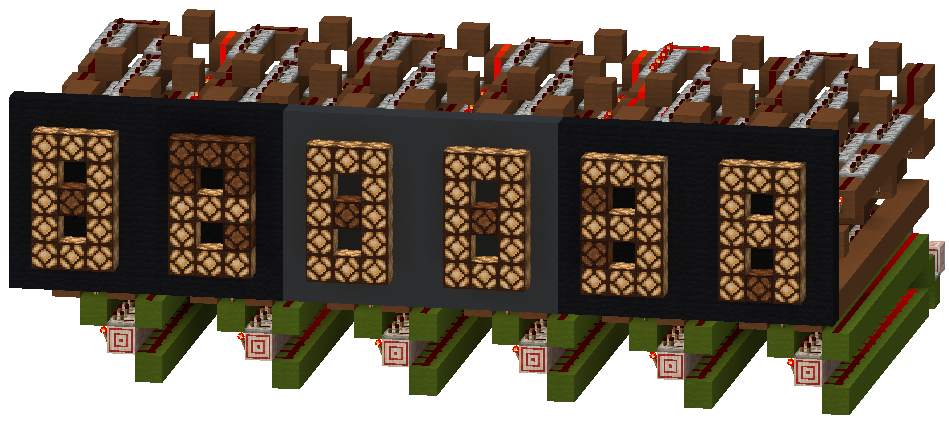
\includegraphics[width=\textwidth]{imgs/screen.png}
				\caption*{$7$-segment hex display}
			\end{figure}
		\end{column}
	\end{columns}
\end{frame}

\begin{frame}
	\frametitle{Some stats}

	Performance:
	\begin{itemize}
		\item In-order, single core
		\item $0.1$Hz clock (on normal game speed)
		\item $1$ IpC
	\end{itemize}

	The actual circuit
	\begin{itemize}
		\item $70$k blocks
		\item $3.6$k registers/repeaters
		\item $30$k unit lengths of wiring
	\end{itemize}
\end{frame}

\begin{frame}[fragile]
	\frametitle{Toolchain}
	\begin{columns}
		\begin{column}{0.4\textwidth}
			\begin{itemize}
				\item Assembler
			\end{itemize}
			\lstdefinelanguage{asm}
			{morekeywords={add, xor, jmp, jneg, loadi},
				sensitive=true,
				morecomment=[l]{--},
				morecomment=[s]{/*}{*/},
			}
			\lstset{language=asm}
			\begin{lstlisting}
.sec
	add %5 %2 %2
	xor %2 %1 %9
	add %5 %9 %9
	add %6 %9 %0
	jneg min
	jmp print_sec
.min
	loadi $0 %2
	add %5 %3 %3
	xor %3 %1 %9
    ...
	\end{lstlisting}
		\end{column}
		\pause
		\begin{column}{0.6\textwidth}
			\begin{itemize}
				\item Linker
			\end{itemize}
			Resolves label references and computes jumps
			\lstset{language=asm}
			\begin{lstlisting}
add %5 %2 %2
xor %2 %1 %9
add %5 %9 %9
add %6 %9 %0
jneg 0x10
jmp 0x03
...
	\end{lstlisting}
			\pause
			\begin{itemize}
				\item ROM generator
			\end{itemize}
			\lstdefinelanguage{command}
			{morekeywords={setblock, torch, air},
				sensitive=true,
				morecomment=[l]{--},
				morecomment=[s]{/*}{*/},
			}
			\lstset{language=command}
			\begin{lstlisting}
setblock -272 197 -1402 torch
setblock -270 197 -1402 torch
setblock -268 197 -1402 air
...
    \end{lstlisting}
		\end{column}
	\end{columns}
\end{frame}

\section{Demo}

\begin{frame}
	\frametitle{The Demo}
	% TODO the link?
	Link on \url{\rvlink}

	%clock
	%e approximation using RNG
	%joke: very secure because: active temper detection with TNT + industry grade (aka. java) RNG.
\end{frame}

\section{The community}

\begin{frame}
	\frametitle{The community}
	\framesubtitle{Other CPU designs}

	\textbf{O}pen \textbf{R}edstone \textbf{E}ngineers
	\url{https://openredstone.org/}

	
\includegraphics[width=0.2\textwidth]{imgs/ore.png}

	\begin{itemize}

		\item Shared circuit designs
		\item Collaborative building
		\item ``school'' system
		\item Guides and resources
		\item Guest lecture at Harvard \url{https://www.youtube.com/watch?v=EcGExRlHVzg}
	\end{itemize}
\end{frame}

\begin{frame}
	\frametitle{The community}
	\framesubtitle{Open-source tools}

	In addition to shared circuit designs and techniques:

	\begin{itemize}
		\item Alternative high-performance Minecraft servers (\url{https://github.com/MCHPR/MCHPRS})
		\item Game mods for debugging
		\item Community-organization tools
	\end{itemize}

	All in all, very similar to traditional FOSS comunities.

\end{frame}

\begin{frame}
	\frametitle{Community showcase}
	\center
	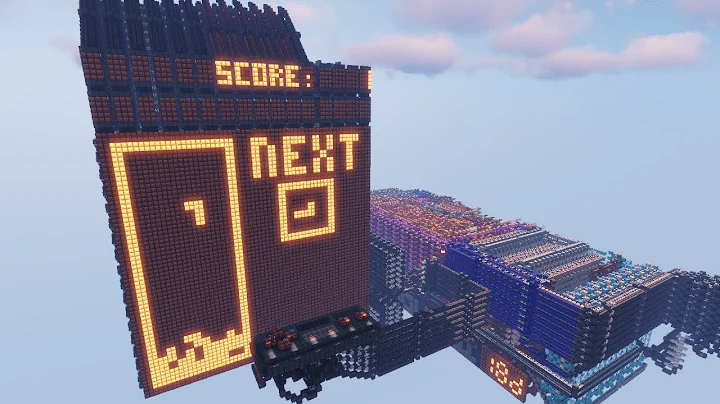
\includegraphics[width=0.6\textwidth]{imgs/chungus.png}
	\url{https://github.com/sammyuri/chungus-2-assembler}

	$1$Hz, $4$-stage pipeline, \hw{} \texttt{mult} \& \texttt{div}, instruction
	and data cache, \hw{} callstack

	Toolchain: MIT license
\end{frame}

\section{Verification}
% \begin{frame}
% 	\frametitle{Perspectives}
% 	\begin{itemize}
% 		\item arm cortex A53
% 		\item RV32-I
% 		\item dynamic FPGA
% 		\item MCHPS
% 		\item semantics and formal verification
% 	\end{itemize}
% \end{frame}

\begin{frame}
	\frametitle{Formal verification}
	\begin{itemize}
		\item Existing tools do not know Minecraft
		\item Define Minecraft's semantics
	\end{itemize}
\end{frame}

\begin{frame}
	\frametitle{First attempt: k-induction with Haskell}
	\begin{itemize}
		\item Export the matrix of blocks
		\item Graph representation % explain why
		\item Define Minecraft's semantics
		\item DSL to express the goal
		\item Z3 SMT solving
	\end{itemize}

	Subset of the ALU verified!

	CPU parts list:
	\begin{itemize}
		\item 7k redstone elements
		\item 30k redstone wires
	\end{itemize}

	so, probably too slow anyways...
\end{frame}

\begin{frame}
	\frametitle{On going second attempt: model checking}
	\begin{figure}
		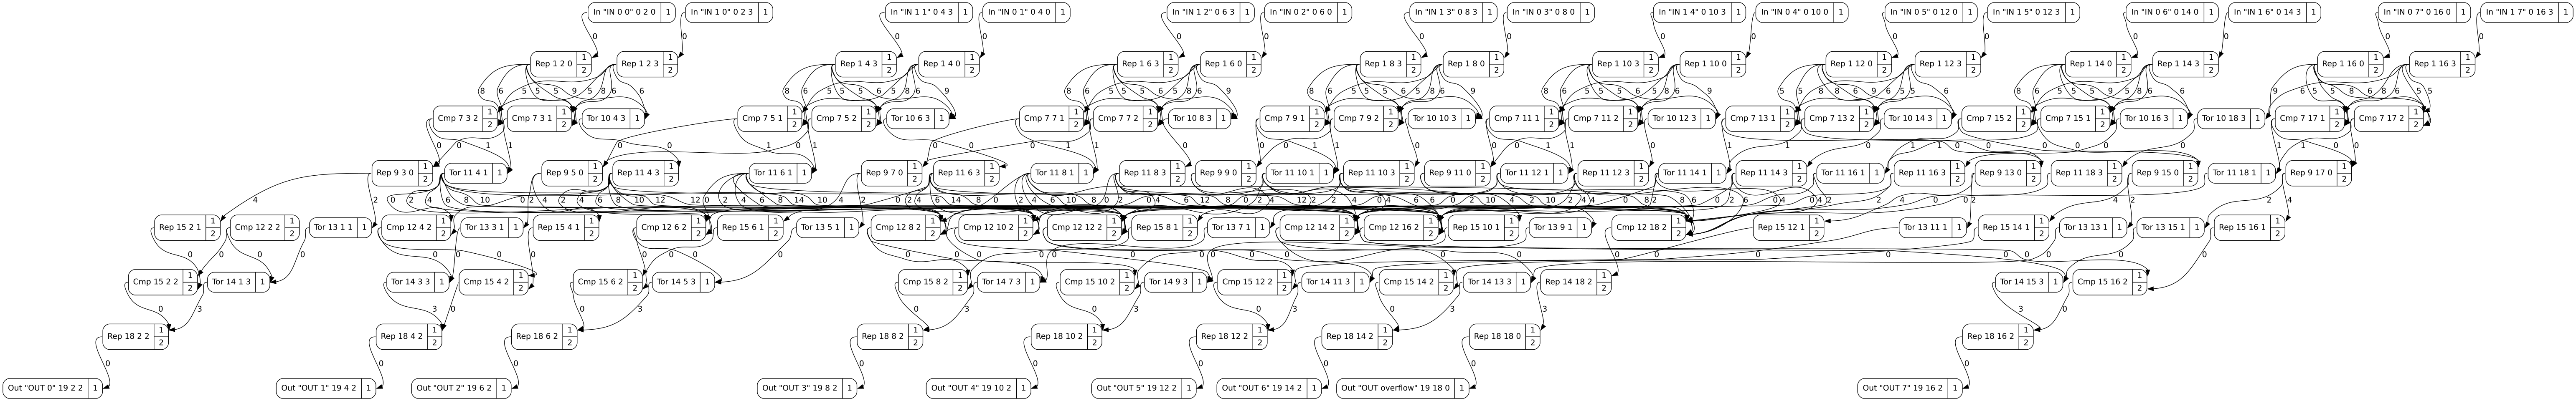
\includegraphics[width=\linewidth]{imgs/cca.png}
		\caption{CCA graph}
	\end{figure}

	Each node is a state machine.

	\begin{itemize}
		\item Model checking
		\item Lean 4 DSL to write semantics and goals
	\end{itemize}
\end{frame}

\section{Educational Aspects}

\begin{frame}
	\frametitle{Learning Outcomes}
	How would you introduce hardware design to a high-schooler?
	\begin{itemize}
		\item FPGA + yosys + nexpnr + git + verilog => blinky
		\item Minecraft with interactive instant feedback
	\end{itemize}
	% easy to understand the parallel nature of hardware
	Just a silly video game? Think again:
	\begin{itemize}
		\item Open Redstone Engineers \href{https://openredstone.org/testimonials}{testimonials}
		\item 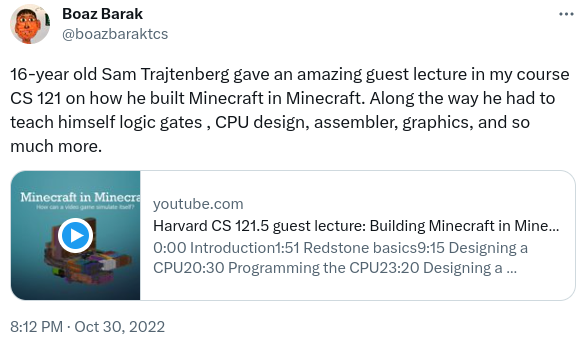
\includegraphics[width=.4\textwidth]{imgs/tweet.png}
		\item Learned from \textbf{first principles}: CPU design, ISA choice, debugging, assembly, linking, and formal verification
	\end{itemize}

	% talent pool to recruit from
\end{frame}

\begin{frame}
	\frametitle{From Minecraft to "real" hardware}
	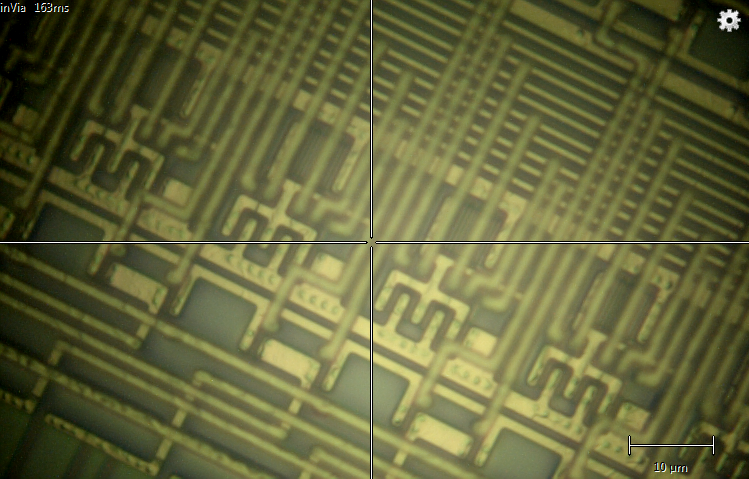
\includegraphics[width=.4\textwidth]{imgs/1000.png}
	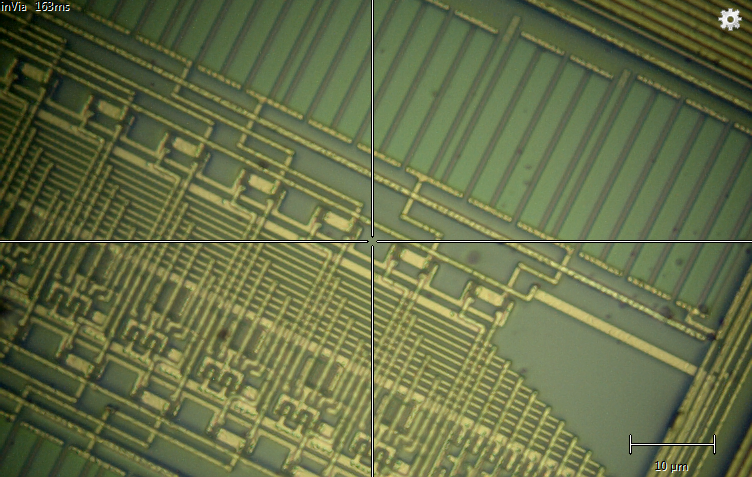
\includegraphics[width=.4\textwidth]{imgs/500.png}
	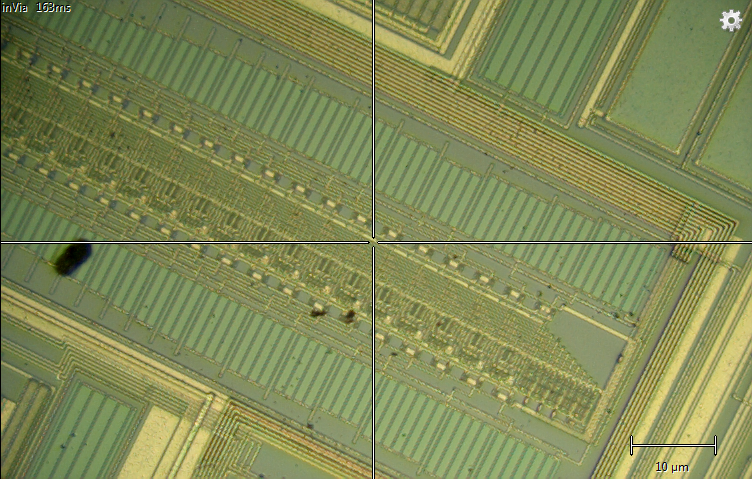
\includegraphics[width=.4\textwidth]{imgs/200.png}
	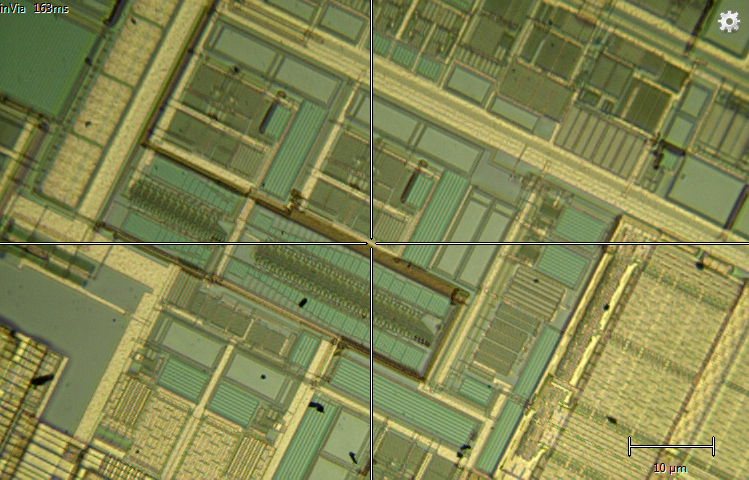
\includegraphics[width=.4\textwidth]{imgs/50.png}
\end{frame}

\begin{frame}
	\frametitle{Acknowledgement}
	\begin{columns}
		\begin{column}{0.5\textwidth}
			Special thanks to friends and collaborators who helped us on this project,
			including:
			\begin{itemize}
				\item Hadrien Barral
				\item Rémy Citerin
			\end{itemize}
		\end{column}
		\begin{column}{0.5\textwidth}
			A big thank you to the FSiC committee for hosting our talk!
			\begin{figure}
				
\includegraphics[width=0.75\textwidth]{imgs/Fsic2023_logo.png}
			\end{figure}
		\end{column}
	\end{columns}
\end{frame}

\begin{frame}[fragile]
	\frametitle{Q/A}
	\begin{columns}
		\begin{column}{0.4\textwidth}
			% TODO Add key points of the talk
			\begin{itemize}
				\item \hw{} design in Minecraft
				\item ISA and implementation
				\item ASM-to-ROM toolchain
				\item Formal verification efforts
				\item FOSS Minecraft engineers community
			\end{itemize}
		\end{column}
		\begin{column}{0.6\textwidth}
			\begin{center}
				Craft your IC project wiki page
				\\ \url{\rvlink}
				\begin{figure}
					\qrcode[height=4cm]{\rvlink}
				\end{figure}
			\end{center}
		\end{column}
	\end{columns}
	\begin{center}
		\small \names{}
	\end{center}
\end{frame}

\begin{frame}
	\frametitle{Minecraft HDL efforts}
	\begin{center}
		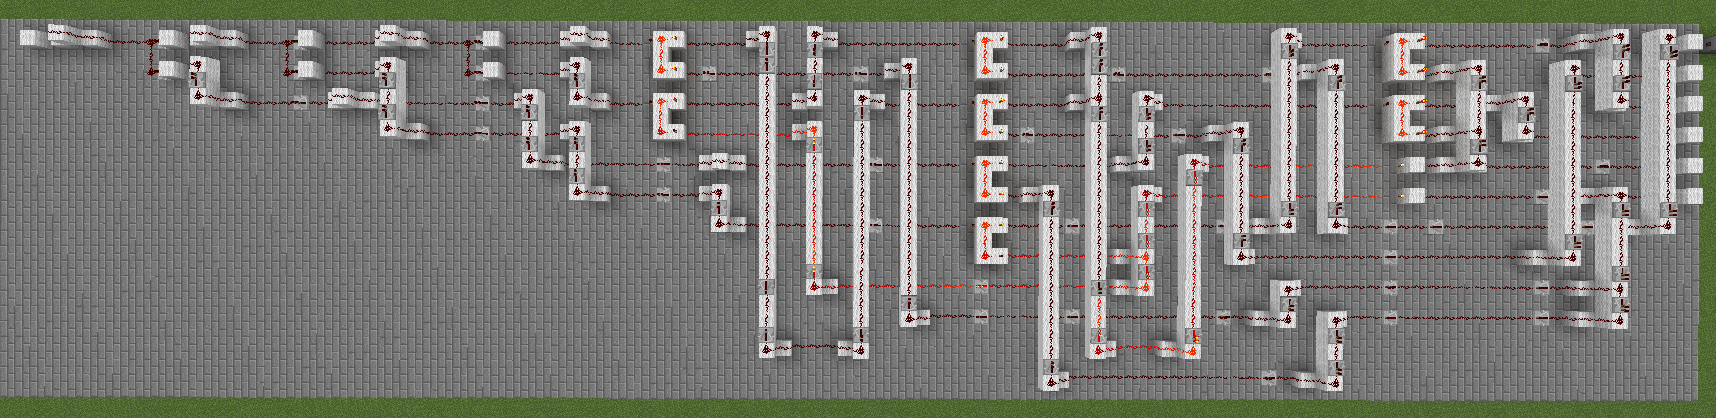
\includegraphics[width=\textwidth]{imgs/hdl.png}
		\url{https://github.com/itsFrank/MinecraftHDL}
	\end{center}
\end{frame}

\begin{frame}
	\frametitle{Minetest}
	A FOSS Minecraft clone, with strong education goals. Licensed under LGPL$2.1$

	\begin{center}
		
\includegraphics[width=0.3\textwidth]{imgs/minetest.pdf}
		\url{https://www.minetest.net}
	\end{center}
\end{frame}

\newpage
\bibliographystyle{plain}
\bibliography{ref}

\end{document}
